\documentclass{article}
\usepackage{amsmath, amssymb}
\usepackage{graphicx}
\usepackage{booktabs}
\usepackage{geometry}
\usepackage{natbib}

% Set up the geometry for better margins
\geometry{margin=1in}

% Title, author, and date
\title{Sample Academic Paper Using LaTeX and BibTeX}
\author{Kong Wangyang\\
University of Connecticut}
\date{\today}

\begin{document}

\maketitle

\begin{abstract}
This is a sample manuscript created using LaTeX to demonstrate the proper use of typesetting for academic papers. It includes references to various sections, tables, figures, and equations, with citations using BibTeX. This template showcases essential components of a research paper.
\end{abstract}

\section{Introduction}
This document demonstrates how to properly use LaTeX for typesetting a statistical paper. The main content will guide you through the basics of sections, citations, tables, figures, and equations. 

At the end of this introduction, we provide a roadmap to guide readers through the paper. Section \ref{sec:methods} describes the methods used, including key equations. Section \ref{sec:results} presents the results, including a table and a figure for illustration. Finally, Section \ref{sec:conclusion} offers concluding remarks and future directions.

\section{Methods} \label{sec:methods}
In this section, we introduce the main methods used in our research. Consider the basic mathematical operation of integration, which is a fundamental tool in statistical modeling:
\begin{equation}
    \int_a^b f(x) \, dx = F(b) - F(a). \label{eq:integration}
\end{equation}
Equation \eqref{eq:integration} shows the definite integral of a function $f(x)$ from $a$ to $b$. Integration plays a significant role in many statistical procedures, such as in calculating areas under curves, which is vital in probability and statistics.

Another critical aspect is hypothesis testing, where we test a null hypothesis $H_0$ against an alternative hypothesis $H_1$. For instance, the $t$-test is often used:
\[
    t = \frac{\bar{X} - \mu}{S / \sqrt{n}}.
\]
Here, $\bar{X}$ is the sample mean, $\mu$ is the population mean, $S$ is the sample standard deviation, and $n$ is the sample size. The variance of the data is given by $\sigma^2 = \frac{1}{n-1} \sum_{i=1}^{n} (x_i - \bar{x})^2$, highlighting the distribution spread.

\section{Results} \label{sec:results}

Table \ref{tab:sample} shows a summary of the data used in the analysis. Data tables should always be well-labeled, and values should be rounded to appropriate decimal places.

\begin{table}[htbp]
    \centering
    \caption{Summary Statistics of the Sample Data}
    \begin{tabular}{lcc}
        \toprule
        Variable & Mean & Standard Deviation \\
        \midrule
        $X_1$ & 10.5 & 2.3 \\
        $X_2$ & 15.8 & 4.1 \\
        \bottomrule
    \end{tabular}
    \label{tab:sample}
\end{table}

Figure \ref{fig:sample} shows a graphical representation of the data. Graphs help visualize the trends and patterns that might not be evident from the tables. The R script used for generating the sample plot can be found in the code folder named \texttt{generate\_plots.R}.

\begin{figure}[htbp]
    \centering
    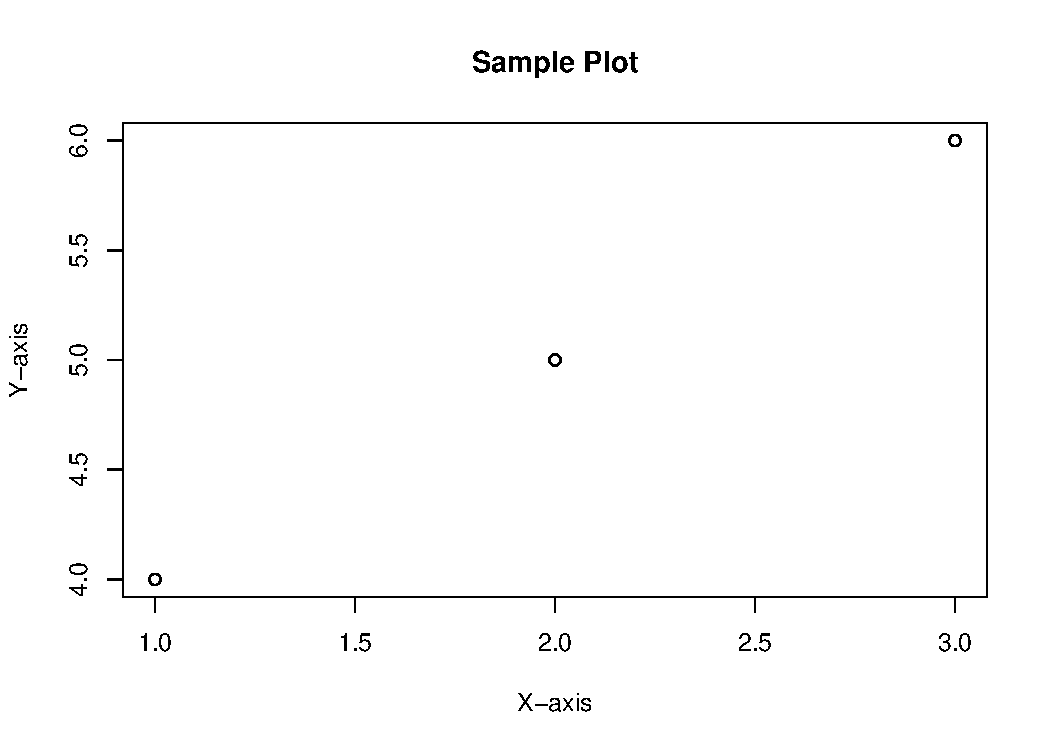
\includegraphics[width=0.6\textwidth]{figures/sample_plot.pdf}
    \caption{A Sample Plot of the Data}

    \label{fig:sample}
\end{figure}

\section{Conclusion} \label{sec:conclusion}
In this paper, we demonstrated how to use LaTeX effectively for academic writing, integrating figures, tables, and equations. Future work could involve expanding on these methods or applying them to specific case studies. This approach aligns with best practices outlined in recent literature \citep{example1}. As discussed by \citet{example2}, using proper typesetting tools can significantly enhance the quality and readability of scientific papers.

\appendix
\section{Appendix}
The appendix provides additional material that is too detailed for the main text, such as extended data tables, supplementary figures, or additional mathematical derivations.

\newpage
\bibliographystyle{plainnat}
\bibliography{references}

\end{document}
